\documentclass[conference]{IEEEtran}

% *** MISC UTILITY PACKAGES ***
%


% *** CITATION PACKAGES ***
%
\usepackage{cite}

% *** GRAPHICS RELATED PACKAGES ***
%
\usepackage[pdftex]{graphicx}
% declare the path(s) where your graphic files are
\graphicspath{{./images/}}
\DeclareGraphicsExtensions{.pdf,.jpeg,.png}

% *** MATH PACKAGES ***
%
\usepackage[cmex10]{amsmath}

% *** SPECIALIZED LIST PACKAGES ***
%
\usepackage{algorithmic}

% *** ALIGNMENT PACKAGES ***
%
\usepackage{array}


% *** SUBFIGURE PACKAGES ***
\usepackage[cpation=false,font=footnotesize]{subfig}

% *** FLOAT PACKAGES ***
%

% *** PDF, URL AND HYPERLINK PACKAGES ***
%
\usepackage{url}


% correct bad hyphenation here
\hyphenation{}


\begin{document}
%
% paper title
\title{Wall following and obstacle avoidance with SARSA $\lambda$ Reinforcement Learning}


% author names and affiliations
\author{\IEEEauthorblockN{Matthew J. Urffer}
\IEEEauthorblockA{Department of Nuclear Engineering \\
University of Tennessee \\
Knoxvilee, Tennessee, 37916 \\
Email: matthew.urffer@gmail.com
}}



% make the title area
\maketitle


\begin{abstract}
\boldmath
Reinforcment learning is a learning process in which an agent is reward for making the correct actions at a particular state. 
This learning strategy is extremely useful in complex enviorments that are difficult to modeled, or ones in which the assement of an action is delayed.
This work attempts to implement a reinforcment learning strategy for a wall-following and obstacle avoidance robot in the player stage enviorment.
Attempts were maed to implement reinforcment learning using the SARSA $\lambda$ algorthim with an $\epsilon$ greedy policy and eligibility traces, but utimately these attempts did not result in a convergent implementation.
In this implementation a dscritized state space was utilized as well as a discritized action space.
\end{abstract}
\IEEEpeerreviewmaketitle



\section{Introduction}

Reinforcement learning is a popular learning strategy for which direct supervision of the agent is not possible. 
Reinforcement learning is often formulated as a problem of trying to find the action that an agent can take in some enviroment in order to maximize a reward.
Rather than learning a particular solution to the problem, Reinforcement learning can bet thought as attempting to find a policy for solving the problem.  

\subsection{Reinforcment Learning}
A basic reinforcement learning problem is defined by:
\begin{itemize}
    \item a set of states $S$,
    \item a set of actions $A$,
    \item transitions between states,
    \item a reward function,
    \item and some terminal states.
\end{itemize}
Reinforcement learning algorthims then define an agent which goes out in the enviroment and is trained to complete the learning. 
The \emph{agent} in reinforcemnt must complete the following:
\begin{itemize}
	\item find out the \emph{state} of the environment,
	\item take \emph{actions} to modify the enviroment,
	\item determine if the \emph{goal} has been acheived.
\end{itemize}
The agent then interacts within the enviroment in order to achieve a goal.  In reinforcemnt learning this is broken into four sections:
\begin{itemize}
	\item a \emph{policy} which maps between a state and and action that the agent can preform,
	\item a \emph{reward function} which defines the goal of the agent,
	\item a \emph{value function} which determines how profitable it is to be in a given state (in relationship to achieving the award)
	\item and a \emph{enviroment} which determines the states and actions that can be completed.
\end{itemize}

\begin{figure}
\centering
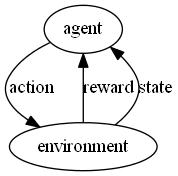
\includegraphics[width=2.5in]{RLDiagram}
\caption{Reinforcement Learning Process}
\label{RLDiagram}
\end{figure}

\section{Methods}
\subsection{Problem Formulation}
The problem was formulated as a wall following and obsticale avoidance problem in which it was desired to have the robot follow at least $d_{wall} = 0.75 \text{m}$ from a wall, and for the robot to come no closer than $d_{obsticale} = 0.25 \text{m}$ from an obsticle.
The player-stage simulation envioroment (a well known robicitics simultiont package) was choosen to simulate the actions and enviroments.  The states were discrizied into a minimum left distance, a minimum right distance, and the distance to the closest object.
\subsection{SARSA $\lambda$}

\subsection{Exploration vs. Explotation}
Reinforcement learning algorthims have to balance exploration (determining the rewards of new actions) vs exploation (chosing the action that previously had the best reward). For this implemenation an $\epsilon$-greedy policy was choosen; for probability $\epsilon$ the action was choosen to exploate the previous knowledge of the solution (i.e.e the previous best action), but for probability $1-\epsilon$ a random action was choosen.
\section{Future Work}
It is acknowledged that
\begin{itemize}
	\item What happens if we expand the discreitization
	\item Can we make two policies, one for avoidance and one for wall following
\end{itemize}


% An example of a double column floating figure using two subfigures.
% (The subfig.sty package must be loaded for this to work.)
% The subfigure \label commands are set within each subfloat command, the
% \label for the overall figure must come after \caption.
% \hfil must be used as a separator to get equal spacing.
% The subfigure.sty package works much the same way, except \subfigure is
% used instead of \subfloat.
%
%\begin{figure*}[!t]
%\centerline{\subfloat[Case I]\includegraphics[width=2.5in]{subfigcase1}%
%\label{fig_first_case}}
%\hfil
%\subfloat[Case II]{\includegraphics[width=2.5in]{subfigcase2}%
%\label{fig_second_case}}}
%\caption{Simulation results}
%\label{fig_sim}
%\end{figure*}
%
% Note that often IEEE papers with subfigures do not employ subfigure
% captions (using the optional argument to \subfloat), but instead will
% reference/describe all of them (a), (b), etc., within the main caption.


% An example of a floating table. Note that, for IEEE style tables, the 
% \caption command should come BEFORE the table. Table text will default to
% \footnotesize as IEEE normally uses this smaller font for tables.
% The \label must come after \caption as always.
%
%\begin{table}[!t]
%% increase table row spacing, adjust to taste
%\renewcommand{\arraystretch}{1.3}
% if using array.sty, it might be a good idea to tweak the value of
% \extrarowheight as needed to properly center the text within the cells
%\caption{An Example of a Table}
%\label{table_example}
%\centering
%% Some packages, such as MDW tools, offer better commands for making tables
%% than the plain LaTeX2e tabular which is used here.
%\begin{tabular}{|c||c|}
%\hline
%One & Two\\
%\hline
%Three & Four\\
%\hline
%\end{tabular}
%\end{table}



\section{Conclusion}
Reinforcement learning has been proven as a techinque of learing a policy necessary to achieve a goal. 
Reinforcement learning (using the SARSA $\lambda$ algorthim) was attempted to be implemented in the player-stage enviroment in order to teach a robot the optimal policy to avoid walls and to avoid obstalces.
While the particular implementation was not successful at achieveing this goal, the general 
The conclusion goes here.



% use section* for acknowledgement
\section*{Acknowledgment}
Once again I would like to thank Matthew Lish for his help.  His support and insight is gratefully acknowledgment.


% trigger a \newpage just before the given reference
% number - used to balance the columns on the last page
% adjust value as needed - may need to be readjusted if
% the document is modified later
%\IEEEtriggeratref{8}
% The "triggered" command can be changed if desired:
%\IEEEtriggercmd{\enlargethispage{-5in}}

% references section

% can use a bibliography generated by BibTeX as a .bbl file
% BibTeX documentation can be easily obtained at:
% http://www.ctan.org/tex-archive/biblio/bibtex/contrib/doc/
% The IEEEtran BibTeX style support page is at:
% http://www.michaelshell.org/tex/ieeetran/bibtex/
%\bibliographystyle{IEEEtran}
% argument is your BibTeX string definitions and bibliography database(s)
%\bibliography{IEEEabrv,../bib/paper}
%
% <OR> manually copy in the resultant .bbl file
% set second argument of \begin to the number of references
% (used to reserve space for the reference number labels box)
\begin{thebibliography}{1}

\bibitem{IEEEhowto:kopka}
H.~Kopka and P.~W. Daly, \emph{A Guide to \LaTeX}, 3rd~ed.\hskip 1em plus
  0.5em minus 0.4em\relax Harlow, England: Addison-Wesley, 1999.

\end{thebibliography}




% that's all folks
\end{document}


